\documentclass[12pt]{article}
\usepackage[utf8]{inputenc}
\usepackage{spverbatim}
\usepackage{algorithmic}
\usepackage{amsmath}
\usepackage{amsthm}
\usepackage{amssymb}
\usepackage{amsfonts}
\usepackage[margin=1in]{geometry}
\usepackage{graphicx} 
\usepackage{hyperref}
\graphicspath{ {images/} }
\setlength{\parskip}{\baselineskip}%
\setlength{\parindent}{0pt}%
\graphicspath{ {images/} }
\title{Probability and Statistics \\ Assignment R}
\author{Hien Le - hien.le@student.auc.nl \\ Deniz Ovalioglu - deniz.ovalioglu@student.auc.nl}
\date{March 2018}

\begin{document}
\maketitle

\subsection*{Exercise R.1}
Suppose a coin is flipped repeatedly for which the probability of
heads is $p = 0.3$. Different flips of the coin are independent. In what follows, $X_{n}$ denotes the number of heads obtained after $n$ flips.

(a) Based on the frequency interpretation of the concept “probability”, what value would you expect $X_{n}$ to have when $n$ is large?
\subsubsection*{Answer}
Based on the description of $X_{n}$, we can deduce that $X_{n}$ has a Binomial distribution i.e. $X_{n} \sim Bin(n, 0.3)$. Therefore, when $n$ is large, the expectation of $X_{n}$ will be 0.3$n$. The reasoning can be seen in the calculation below, which applies the expectation of each random variable having the Poisson Distribution:\\
Let $X \sim Bin(n,p)$, when $n$ is large, $X \sim E(X) = E\Sigma^{n}_{i=1}X_{i} = \Sigma^{n}_{i=1}E(X_{i}) = np$.

(b) Simulate in R a series of 500 coin flips. Make a plot of $X_{n}$ against $n$, for $n = 1, . . . , 500$. Use \texttt{type="l"} for plotting. Add to this plot the line $np$ against $n$, in a different color.
Hint: A series of 500 independent coin flips can be generated by the R-
command \texttt{x=rbinom(500,1,p)}. The R-function \texttt{cumsum} can be useful when you determine the number of heads after n flips.
\subsubsection*{Answer}
Computation can be seen in Appendix for Exercise R.1.\\
Plot:

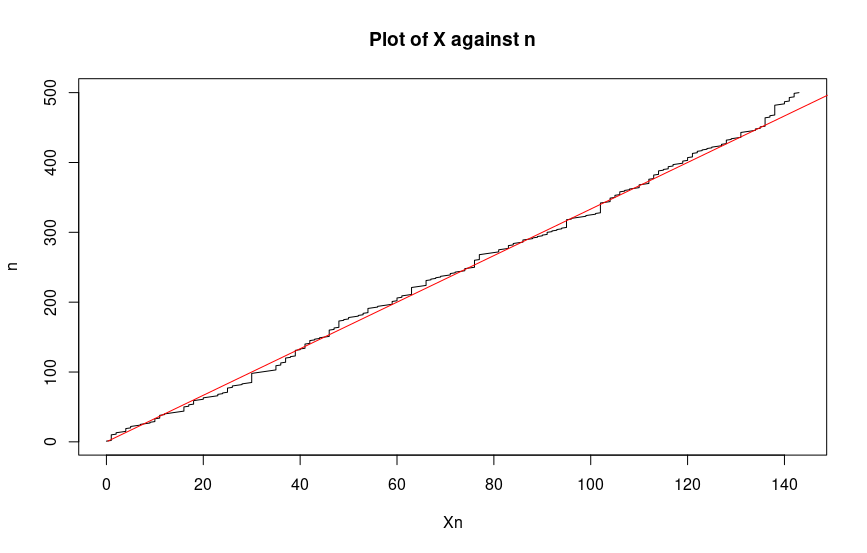
\includegraphics[width=\textwidth]{Ex1Plot1}

(c) Investigate how close the two graphs you produced in part (b) are, relative to their height. That is, for every $n$, compute the relative error $\frac{|X_{n} - np|}{np}$. What happens to the relative error as the number of flips grows? Is this in accordance with your expectations in part (a)?
\subsubsection*{Answer}
Plot:

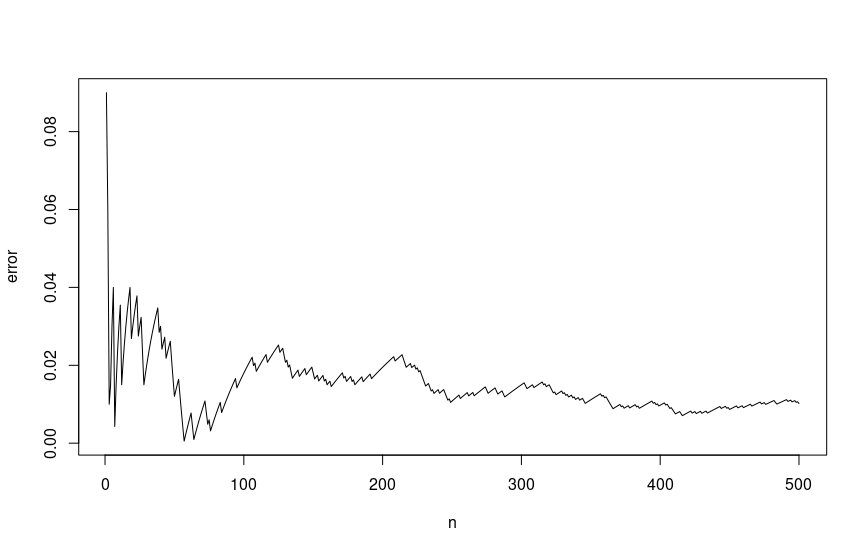
\includegraphics[width=\textwidth]{Ex1Plot2}
The computation of the errors (element-wise) can be seen in the Appendix of Exercise R.1.

Looking at the plot above, it can be concluded that the error, or the (scaled) difference between $np$ and $X_{n}$ reduces as the number of flips grows. This is in accordance with part (a), which claims that as $n$ becomes large, the value of $X_{n}$ eventually reaches $np$.

\subsection*{Exercise R.2}
(a) Make exercise 2.18 (a)–(d) of the book using R (do not use the Normal table). \\Now simulate in R six random samples from $N(3, 16)$: two of size 20, two of size 100, two of size 1.000.\\
(b) Determine for each of the six samples:\\
- the proportion of values that are smaller than 7;\\
- the proportion of values larger than -2;\\
- the 0.95-sample quantile, i.e. the smallest value in the sample for which it holds that at most 5\% of the data in the sample is larger than or equal to this value (use the R-function quantile with \texttt{type=1}).\\
- the proportion of values larger than or equal to 0 and smaller than 4.

Present your results of parts (a) and (b) together in one table. Round all the values to three decimal places.

\subsubsection*{Answer}
(See Table 1)                                                                               

\begin{table}
\centering
\caption{R.2.a and R.2.b}
\begin{tabular}{|c|c|c|c|c|c|c|c|}
\hline
\multicolumn{1}{|l|}{}                                                                                 & \textbf{2.18} & $n=20(1)$ & $n=20(2)$ & $n=100(1)$ & $n=100(2)$ & $n=1000(1)$ & $n=1000(2)$ \\ \hline
\textbf{\textless 7}                                                                                   & 0.841             & 0.933             & 0.928             & 0.826             & 0.792             & 0.832             & 0.844             \\ \hline
\textbf{\textgreater -2}                                                                               & 0.894             & 0.919             & 0.811             & 0.894             & 0.870            & 0.889             & 0.891             \\ \hline
\textbf{\begin{tabular}[c]{@{}c@{}}0.95-sample\\  quantile\end{tabular}}                               & 9.579             & 7.210             & 7.725             & 9.687             & 10.329            & 9.895             & 9.604             \\ \hline
\textbf{\begin{tabular}[c]{@{}c@{}}Larger than\\  or equal \\ to 0 and\\  smaller than\\ 4\end{tabular}} & 0.372             & 0.478             & 0.392             & 0.360             & 0.323             & 0.361             & 0.372             \\ \hline
\end{tabular}
\end{table}

(c) Compare your results for the six samples of part (b) to each other and to the corresponding answers of part (a). Briefly comment on your findings.

\subsubsection*{Answer}
When the results of the six samples are compared to each other, it is clear that the portion smaller than 7 decreases as the sample size increases and this applies to also the portion larger than -2, larger than or equal to 0 and smaller than 4, as well (although there exists a a twist to this increase when samples 2, 3 and 4 are compared individually). Meanwhile, there is an increase in the 0.95-sample quantile value, as the sample size grows. \\
These patterns emerge due to the fact that \textbf{as the sample size grows}, the distribution becomes denser, with more and more values concentrating in the 0.95-quantile range, while values in the range of one-sigma away from the mean become more and more spread out.  \\
When the results of the six samples are compared to the answers in part a, it is observed that the samples 1 and 2 with the size 20 give the furthest answers compared to samples 3, 4, 5, and 6. When Samples 3, 4, 5, and 6 are compared to the answers in a, it is obvious that sample size 1000 shows the closest value. This supports the claim that the sampling distribution approaches a normal distribution as the sample size $n$ increases.

(d) For each of the six samples, draw the scaled histogram and draw the probability density function of $N(3, 16)$ on top of it. Present the six plots in one figure. Briefly comment on what you see in the plots.\\
Hint: The p.d.f. of a normal distribution in R is the function \texttt{dnorm}.

\subsubsection*{Answer}

The 6 plots can be seen below, in the order of left to right, top to bottom (and computation is put in Appendix for Exercise R.2):\\

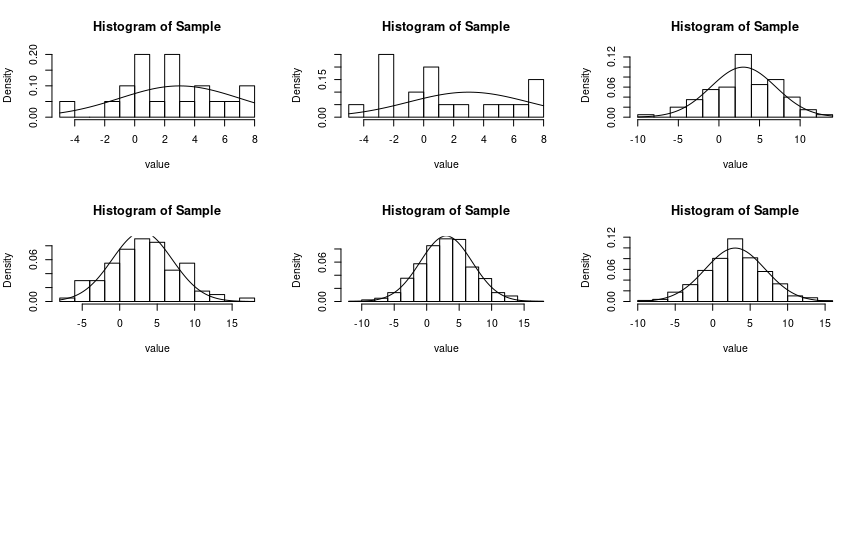
\includegraphics[width=\textwidth]{Ex2AllPlots}

(e) Which common phenomenon do your findings in parts (c) and (d) illustrate?

\subsubsection*{Answer}

Both (c) and (d) illustrate the fact that the larger the sample size, the closer the histogram is with the density curve of the $N(3,16)$ distribution i.e. the larger the sample size, the closer the distribution is to a normal distribution.
\subsection*{Exercise R.3}
In this exercise, you will estimate an unknown probability by the frequency of occurrence of the event in a long series of experiments. Assume that birthdays are uniformly spread over a year of 365 days, and that $n$ students are chosen at random independently from each other. \\ Consider the event $A_{n}$ = \{there is a day (at least one) in the year when at least 3 out of the $n$ chosen students have their birthday\}.

(a) Write a function that estimates $P\{A_{n}\}$ by simulating 100 experiments (that is, by taking 100 samples of size $n$) and finding out for each experiment (that is, for each sample) if $A_n$ occurs. Take $n$ as the argument of the function.\\
Hint: Use a for-loop.
\subsubsection*{Answer}
See Appendix for Exercise R.3

(b) Create a vector \texttt{prob} that consists of the estimates for the probabilities $P\{A_{n}\}$ for $n = 1, 2, . . . , 200$. Plot these probabilities against $n$.normal distribution.
\subsubsection*{Answer}
Computation can be seen in appendix for Exercise R.3.\\
Plot:

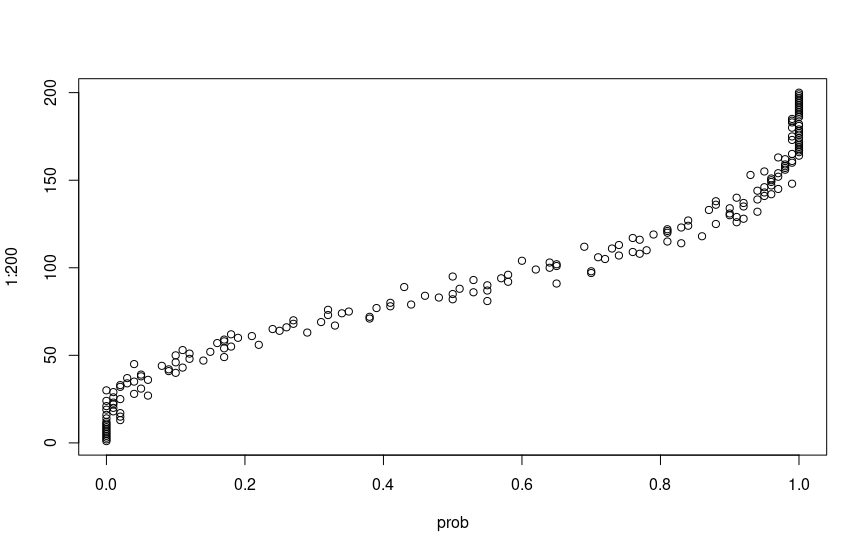
\includegraphics[width=\textwidth]{Ex3Plot1}

(c) Estimate the number of students that should be chosen so that the probability of the event $A_{n}$ is at least 70\% by finding the smallest $n$ such that prob[$n$] $\geq$ 0.7.\\
\subsubsection*{Answer}
Computation can be seen in Appendix for Exercise R.3.\\
The smallest number of subjects that was returned from 100 experiments of 200 students each ($n=200$) was 102 (this value may fluctuate between 101, 102 and 103).

(d) Do you think it is really the case that $P\{A_{n}\} \geq$ 0.7 for the $n$ you found in part (c)? Check your answer by making a new estimate for $P\{A_{n}\}$ based on 10.000 samples and comment.
\subsubsection*{Answer}
For 10,000 samples, the program execution took rather long, but eventually the least $n$ that got output and was 106. This value is relatively close to what are often output in (c).

(e) Take 100 samples of 75 students, and for each sample count on how many days at least 3 students celebrate their birthday simultaneously. Make a histogram of these numbers and calculate the average.
\subsubsection*{Answer}
The average of the vector of number of days (see Appendix of Exercise R.4 for computation) is 1.12.

Plot:

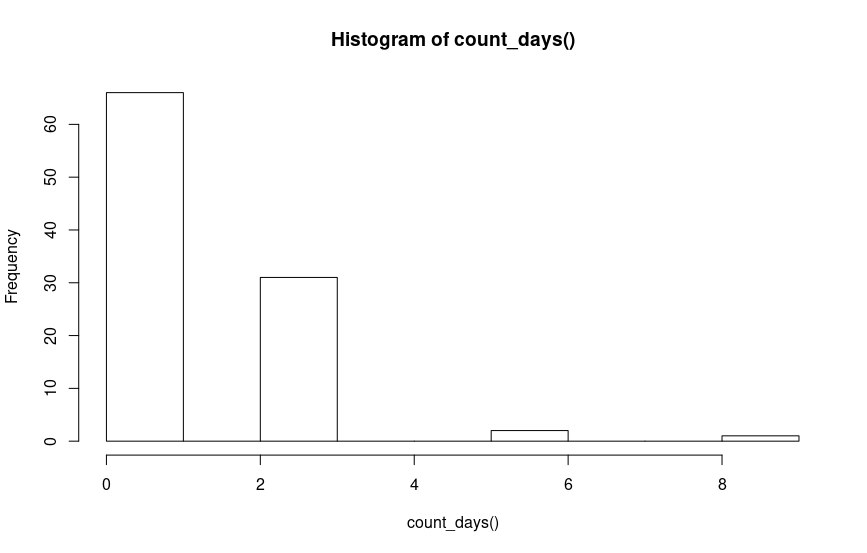
\includegraphics[width=\textwidth]{Ex3Plot2}

(f) Repeat the calculation of part (e) 100 times and make a histogram of the averages. Compare to the histogram from part (e) and comment.
\subsubsection*{Answer}
Plot:

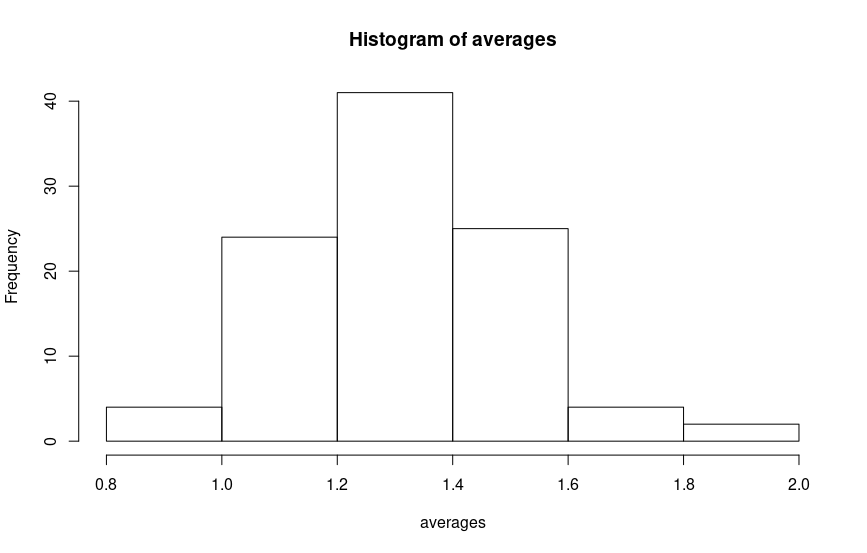
\includegraphics[width=\textwidth]{Ex3Plot3} 

As can be seen, the two diagrams differ greatly. Here, what we are doing is visualising the distribution of the sample means. What we have found out through this histogram of averages is that the sample mean has a normal distribution.

\subsection*{Exercise R.4}
R has commands that generate random variables from many standard distributions. In this exercise, you will learn how to simulate random variables from non-standard distributions. Consider the following c.d.f.:

$F(x) = \frac{e^{x}}{1 + e^{x}}$, $x \in R$

(a) Compute the quantile function $F^{-1}(q), q \in (0, 1)$.
\subsubsection*{Answer}
The quantile function $F^{-1}$ is the inverse of $F(x)$ and can be computed as followed:\\
Let $y= \frac{e^{x}}{1+e^{x}}$\\
$\Leftrightarrow e^{x} = y + e^{x}y$\\
$\Leftrightarrow e^{x}(1 - e^{x}) = y$\\
$\Leftrightarrow e^{x} = \frac{y}{1-y}$\\
$\Leftrightarrow x$ = ln$\frac{y}{1-y}$

Therefore, $F^{-1}(q) =$ ln$\frac{q}{1-q}$.

(b) Simulate a random sample u of size $n = 1.000$ from the uniform distribution on (0, 1). Apply the quantile function $F^{-1}$ to u element-wise and plot a scaled histogram of this transformed vector.\\
Hint: A sample of size n from the uniform distribution on $(a, b)$ can be generated by the R-command \texttt{runif(n,a,b)}.
\subsubsection*{Answer}
Plot (unscaled): 

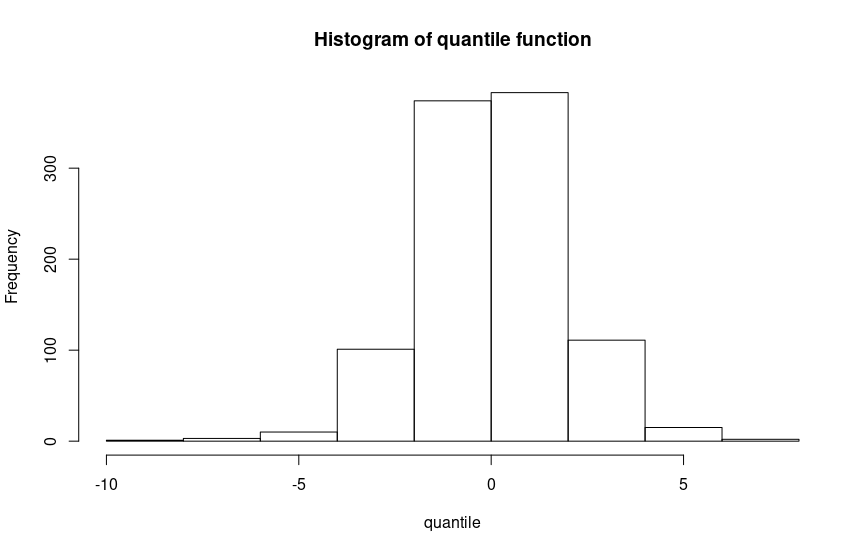
\includegraphics[width=\textwidth]{Ex4Plot1}

Plot (scaled):

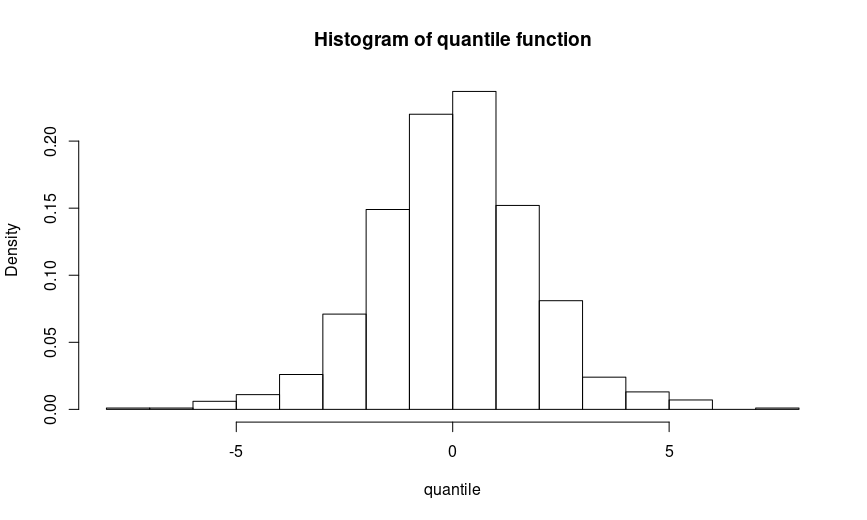
\includegraphics[width=\textwidth]{Ex4Plot2scaled} 

(c) Compute the p.d.f. that corresponds to $F$ and plot it on top of the histogram from (b).
\subsubsection*{Answer}
By definition, we have that $f_{X}(x) = F'_{X}(x)$ at all points $x$ at which $F_{X}$ is differentiable. In this case, $f(x) = F'(x) = \frac{e^{x}(1+e^{x}) - e^{2x}}{(1+e^{x})^{2}} = \frac{e^{x}}{(1+e^{x})^{2}}$

Plot:

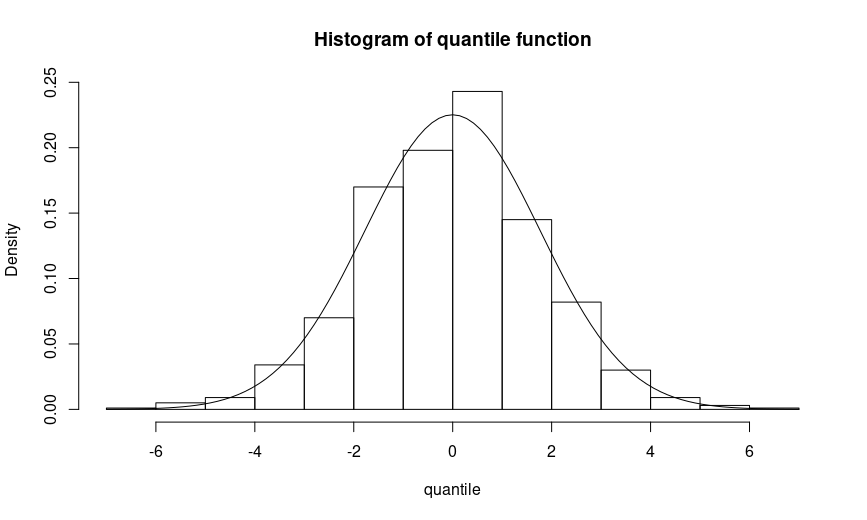
\includegraphics[width=\textwidth]{Ex4Plot2} 


(d) Let a random variable U have uniform distribution on (0, 1). Prove that the c.d.f. of $F^{-1}(U)$ is $F$.\\
Hint: The events $\{F^{-1}(U) \leq x\}$ and $\{F(F^{-1}(U)) \leq F(x)\}$ are the same, why?
\subsubsection*{Answer}
\begin{proof}
Let $X$ = $F^{-1}(U)$. Now, by definition, the \textbf{c.d.f of $F^{-1}(U)$} is $F(F^{-1}(U)) = F_{X}(x)$. We also have $F_{X}(x) = P(X < x)$. Hence, $F(F^{-1}(U)) = P(F^{-1}(U) < x) = P(U < F(x))$ [property of inverse function] $= F(x)$.

The last equality, $P(U < F(x)) = F(x)$, is justified because:\\
$U$ has a uniform distribution on $(0,1)$, the PDF of $U$, $f_{U}(u)$, is therefore 1 for $0 \leq u \leq 1$ and 0 otherwise. Thus, $F_{U}(u) = P(U < u) = \int f_{U}(u) = u$ for $0 \leq u \leq 1$. 
\end{proof}
(e) Based on the previous parts of the exercise, how can you simulate a random variable with the c.d.f. $F$ in R? Which of the previous parts of the exercise proves this approach works and which part illustrates this approach works?

\subsubsection*{Answer}
The first step is to take the inverse of the cdf function with argument $q$ (quantile), which is done in step (a), and next, pass into this argument a uniformly distributed sample. In the previous parts of the exercise, part (d) proves that this approach works - it shows that a random variable $X = F^{-1}(U)$ has a distribution $F$; part (b) and (c) illustrates that this approach works, as the histogram indicates a normal distribution of the quantiles.

(f) Which properties of $F$ enable the approach from (e) to work? Would this approach work for other c.d.f.’s with these properties?
\subsubsection*{Answer}
$F$ must be invertible! The approach would not work otherwise, because then $X$ would not have distribution $F$ any more.

\subsection*{Appendix}

\subsubsection*{Exercise R.1}
\begin{verbatim}

# R.1.b
coin_flips = rbinom(500, 1, 0.3)
range_n = 500
generate_plot= function(sample, n, p){
  plot(cumsum(sample), n, xlab="Xn", ylab="n", main="Plot of X against n", type="l")
  lines(n*p, n, col="red", type="l")
}

generate_plot(coin_flips, 1:range_n, 0.3)

# R.1.c
get_relative_error = function(sample, n, p){
  vector_n = c(1:n)
  error_vector = abs(cumsum(sample) - vector_n*p)/vector_n*p
  plot(vector_n, error_vector, xlab="n", ylab="error", type="l")
}

get_relative_error(coin_flips, 500, 0.3)
distribution $F$ any more\end{verbatim}

\subsubsection*{Exercise R.2}
\label{sec:r.2}
\begin{spverbatim}
# R.2.a.a
pnorm(7, mean = 3, sd = 4);

# R.2.a.b
pnorm(-2, mean = 3, sd = 4, lower.tail = FALSE);

# R.2.a.c
qnorm(0.95, mean = 3, sd = 4);

# R.2.a.d
pnorm(4, mean = 3, sd = 4) - pnorm(0, mean = 3, sd = 4);

# R.2.b

# Simulating random samples:
sample1 = rnorm(20, 3, 4)
sample2 = rnorm(20, 3, 4)
sample3 = rnorm(100, 3, 4)
sample4 = rnorm(100, 3, 4)
sample5 = rnorm(1000, 3, 4)
sample6 = rnorm(1000, 3, 4)

# Means of the samples:
mean(sample1) = 2.340795
mean(sample2) = 1.393221
mean(sample3) = 3.135174
mean(sample4) = 3.219025
mean(sample5) = 3.033966
mean(sample6) = 2.945887

# Standard Deviations of the samples:
sd(sample1) = 3.102667
sd(sample2) = 3.847252
sd(sample3) = 4.123312
sd(sample4) = 4.640701
sd(sample5) = 4.126333
sd(sample6) = 4.013080

# Proportion Smaller than 7:
sample 1 : pnorm(7 , mean(sample1), sd(sample1))
sample 2 : pnorm(7 , mean(sample2), sd(sample2))
sample 3 : pnorm(7 , mean(sample3), sd(sample3))
sample 4 : pnorm(7 , mean(sample4), sd(sample4))
sample 5 : pnorm(7 , mean(sample5), sd(sample5))
sample 6 : pnorm(7 , mean(sample6), sd(sample6)

# Proportion Larger than -2:
sample 1 : pnorm(-2, mean(sample1), sd(sample1), lower.tail = FALSE)
sample 2 : pnorm(-2, mean(sample2), sd(sample2), lower.tail = FALSE)
sample 3 : pnorm(-2, mean(sample3), sd(sample3), lower.tail = FALSE)
sample 4 : pnorm(-2, mean(sample4), sd(sample4), lower.tail = FALSE)
sample 5 : pnorm(-2, mean(sample5), sd(sample5), lower.tail = FALSE)
sample 6 : pnorm(-2, mean(sample6), sd(sample6), lower.tail = FALSE)

# 0.95 Quantile: 
sample 1 : quantile(sample1, 0.95, type = 1)
sample 2 : quantile(sample2, 0.95, type = 1)
sample 3 : quantile(sample3, 0.95, type = 1)
sample 4 : quantile(sample4, 0.95, type = 1)
sample 5 : quantile(sample5, 0.95, type = 1)
sample 6 : quantile(sample6, 0.95, type = 1)

# Between 0 and 4:
sample 1 : pnorm(4, mean(sample1), sd(sample1)) - pnorm(0, mean(sample1), sd(sample1))
sample 2 : pnorm(4, mean(sample2), sd(sample2)) - pnorm(0, mean(sample2), sd(sample2))
sample 3 : pnorm(4, mean(sample3), sd(sample3)) - pnorm(0, mean(sample3), sd(sample3))
sample 4 : pnorm(4, mean(sample4), sd(sample4)) - pnorm(0, mean(sample4), sd(sample4))
sample 5 : pnorm(4, mean(sample5), sd(sample5)) - pnorm(0, mean(sample5), sd(sample5))
sample 6 : pnorm(4, mean(sample6), sd(sample6)) - pnorm(0, mean(sample6), sd(sample6))

# R.2.d
draw_hist_curve = function(sam){
  hist(sam, mean(sam), sd(sam), freq=F, breaks=10, name="Histogram of sample");
  curve(dnorm(x, 3, 4), add=T, lwd=1);
}

#draw_hist_curve(sample1)
#draw_hist_curve(sample2)
#draw_hist_curve(sample3)
#draw_hist_curve(sample4)
#draw_hist_curve(sample5)
#draw_hist_curve(sample6)
\end{spverbatim}

\subsubsection*{Exercise R.3}
\label{sec:r.3}
\begin{verbatim}

# R.3.a
birthday_experiments = function(n, expes){
  occurences = 0;
  for(i in 1:expes){
    sam = sample(1:365, n, replace=TRUE);
    event_An = FALSE;
    for(j in sam){
      if(length(which(sam == j)) >= 3){
        event_An = TRUE; 
      }
    }
    if(event_An == T){
      occurences = occurences + 1;
    }
  }
  return(occurences/expes);
}
print(birthday_experiments(200, 100));

# R.3.b
prob = numeric(200);
for(i in 1:200){
  prob[i] = birthday_experiments(i, 100);
}
#print(prob)

plot(prob, 1:200);

# R.3.c
estimate_n = function(n, expes){
  prob = numeric(n);
  least_n = 1;
  for(i in 1:n){
    prob[i] = birthday_experiments(i, expes);
  }
  while(prob[least_n] < 0.7){
    least_n = least_n + 1;
  }
  print(least_n);
}

estimate_n(200, 100);
estimate_n(200,10000);

# R.3.e
count_days = function(){
  vec_days = numeric(100);
  for(i in 1:100){
    sam = sample(1:365, 75, replace=TRUE);
    num_days = 0;
    for(day in sam){
      occurences = length(which(sam==day))
      if(occurences > 2){
        num_days = num_days + 1;
      }
    }
    vec_days[i] = num_days;
  }
  return(vec_days);
}

hist(count_days(), xlab="# days", main="Histogram of # days");
mean(count_days())
# R.3.f
averages = numeric(100);
for(i in 1:100){
  averages[i] = mean(count_days());
}
#hist(averages)

\end{verbatim}
\subsubsection*{Exercise R.4}
\begin{spverbatim}

# R.4.b
unif_sam = runif(1000, 0, 1);
quantiled_func = function(x){
  return(log(x/(1-x)));
}
quantiled_sam = quantile_func(unif_sam);
hist(quantiled_sam, xlab="quantile", freq=F, breaks=10, main="Histogram of quantile function");

#R.4.c
curve(dnorm(x, mean(quantiled_sam), sd(quantiled_sam)), add=T, lwd=1);

\end{spverbatim}
\end{document}